% Provenance (never printed): cycle 3 / 6e "La planete Terre" (structure of
% the globe: crust, mantle, core); see sources/book1/PROVENANCE.md. Book 1,
% grade 6, chapter 4.
% Vocabulary guard: "magma" not before g7.2 ("molten rock"); P and S waves,
% Moho, core--mantle boundary and lithosphere belong to Book 2 (g11): the
% waves are told in prose, never defined; "seismometer" is defined in g7.3.
\chapter{Het binnenste van de Aarde}\label{ch:g6:inside-the-earth}

In het uiterste noordwesten van Rusland, niet ver van de grens met Noorwegen, is tussen verlaten gebouwen een metalen dop op de grond gelast. Daaronder gaat een gat van maar
ongeveer 23~centimeter breed meer dan 12~kilometer recht naar beneden: het
is het diepste gat dat ooit is gegraven. Het boren duurde ongeveer
20~jaar. De boorders hoopten nog dieper te komen, maar onderin was het
\omterm{def:g3:stones-pebbles-sand:rock}{gesteente} ongeveer 180~graden Celsius, bijna twee keer zo heet als
verwacht: de hitte verboog de boorkoppen en de buizen, en het werk stopte
in 1992. Toch ligt het middelpunt van de Aarde meer dan \textbf{500 keer}
dieper dan de bodem van dat gat. Hoe kunnen we weten wat daar beneden is?
% ledger: sciam:kola-depth, sciam:kola-180C, earth:Rmean

\begin{omfigure}
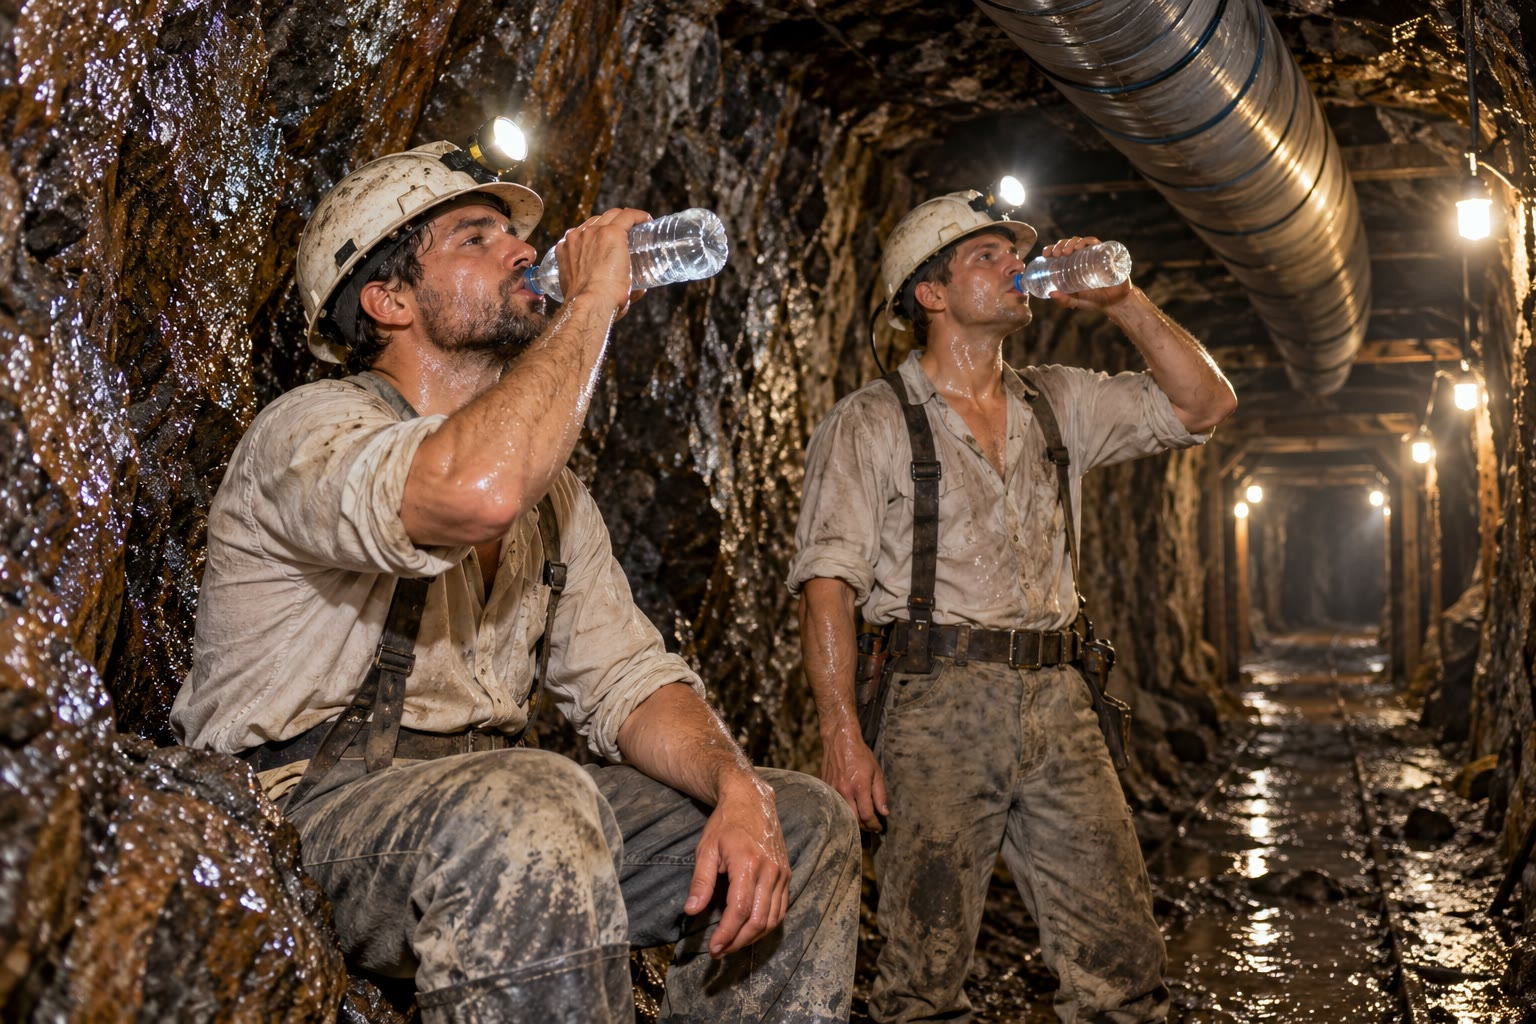
\includegraphics[width=0.62\linewidth]{images/book1/ai/g6-deep-mine.jpg}

{\small Mijnwerkers nemen een slok water in een hete gang, kilometers onder
de grond. (AI-illustratie.)}
\end{omfigure}

\begin{recall}
De Aarde is een \omterm{def:g6:earth-a-planet:planet-types}{rotsplaneet}, een bol met een doorsnede van ongeveer
12\,742~km: haar straal, van het oppervlak tot het middelpunt, is ongeveer
6371~km (\cref{ch:g6:earth-a-planet}). Haar \omterm{def:g3:stones-pebbles-sand:rock}{gesteenten} horen bij drie
families: \omterm{def:g6:rocks-and-minerals:rock-families}{stollingsgesteenten}, \omterm{def:g6:rocks-and-minerals:rock-families}{afzettingsgesteenten} en metamorfe
\omterm{def:g3:stones-pebbles-sand:rock}{gesteenten} (\cref{ch:g6:rocks-and-minerals}). Bij een \omterm{def:g4:volcanoes-earthquakes-first-look:volcano}{vulkaan} komt
gesmolten \omterm{def:g3:stones-pebbles-sand:rock}{gesteente} van onderen omhoog en stroomt het naar buiten als \omterm{def:g4:volcanoes-earthquakes-first-look:eruption}{lava};
bij een \omterm{def:g4:volcanoes-earthquakes-first-look:earthquake}{aardbeving} schudt de grond
(\cref{ch:g4:volcanoes-earthquakes-first-look}).
\end{recall}
% ledger: earth:Rmean

\section{Hoe diep zijn we geweest?}

Mensen graven al heel lang in de Aarde, naar water, steen en metalen. Twee
soorten gaten gaan het diepst.

\textbf{Mijnen.} De diepste mijn ter wereld is een goudmijn bij
Johannesburg, in Zuid-Afrika. De gangen gaan meer dan 4~km onder het
oppervlak. Daar beneden worden de rotswanden ongeveer 60~graden Celsius:
de mijn wordt gekoeld door duizenden tonnen ijs gemengd met water naar
beneden te pompen, en door reusachtige ventilatoren die lucht door de
gangen blazen.
% ledger: gwr:deepest-mine

\textbf{Boorgaten.} Een boorgat is een smal gat dat vanaf het oppervlak
door een machine wordt geboord; er gaat niemand in naar beneden. Het
diepste is het boorgat uit het verhaal aan het begin, geboord voor de
wetenschap op het schiereiland Kola, in het noordwesten van Rusland:
12\,262~meter, dat is ongeveer 12.3~km.
% ledger: sciam:kola-depth

Die diepten lijken enorm. Vergeleken met de grootte van de Aarde zijn ze
piepklein. De figuur hieronder zet ze op één strook, naast de hoogste \omterm{def:g1:landscapes-around-us:landform}{berg},
Mount Everest (8849~m).
% ledger: tht:everest

\begin{omfigure}
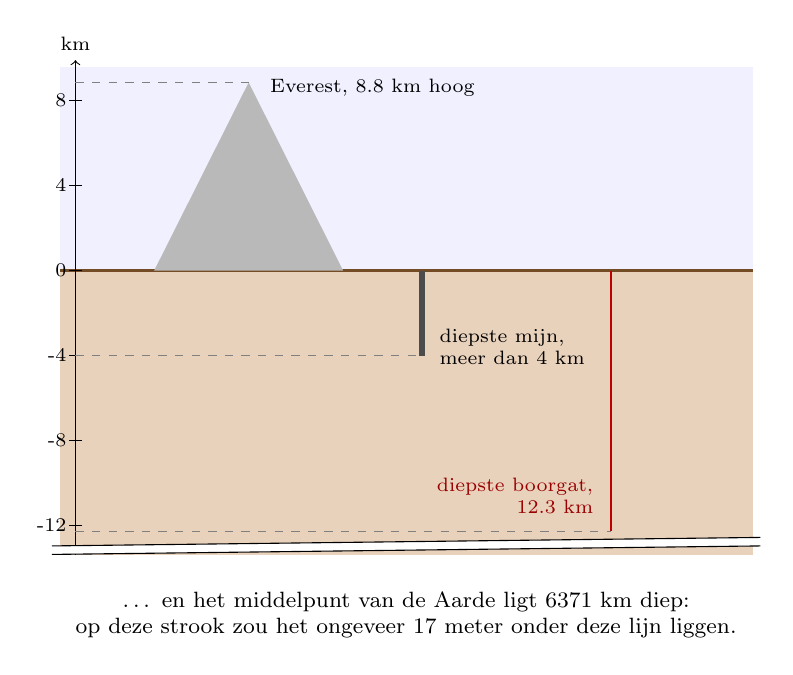
\begin{tikzpicture}[yscale=0.27, xscale=1]
  % sea-level ground and the sky
  \fill[blue!6] (-0.2,0) rectangle (8.6,9.6);
  \fill[brown!35] (-0.2,0) rectangle (8.6,-13.4);
  \draw[thick, brown!60!black] (-0.2,0) -- (8.6,0);
  % depth axis
  \draw[->] (0,-13.4) -- (0,9.9) node[above, font=\scriptsize] {km};
  \foreach \y in {-12,-8,-4,0,4,8} \draw (-0.08,\y) -- (0.08,\y) node[left=2pt, font=\scriptsize] {\y};
  % Everest
  \fill[gray!55] (1.0,0) -- (2.2,8.849) -- (3.4,0) -- cycle;
  \draw[dashed, gray] (0,8.849) -- (2.2,8.849);
  \node[font=\scriptsize, right] at (2.35,8.6) {Everest, 8.8~km hoog};
  % deepest mine
  \draw[line width=2.2pt, black!70] (4.4,0) -- (4.4,-4);
  \draw[dashed, gray] (0,-4) -- (4.4,-4);
  \node[font=\scriptsize, right, align=left] at (4.5,-3.6) {diepste mijn,\\ meer dan 4~km};
  % Kola borehole
  \draw[line width=0.7pt, red!75!black] (6.8,0) -- (6.8,-12.262);
  \draw[dashed, gray] (0,-12.262) -- (6.8,-12.262);
  \node[font=\scriptsize, left, align=right, red!60!black] at (6.7,-10.6) {diepste boorgat,\\ 12.3~km};
  % break and the centre
  \draw[white, line width=3pt] (-0.3,-13.15) -- (8.7,-12.75);
  \draw (-0.3,-13.35) -- (8.7,-12.95);
  \draw (-0.3,-12.95) -- (8.7,-12.55);
  \node[font=\footnotesize, align=center] at (4.2,-16.2) {\ldots\ en het middelpunt van de Aarde ligt 6371~km diep:\\
     op deze strook zou het ongeveer 17~meter onder deze lijn liggen.};
\end{tikzpicture}

{\small Hoogten en diepten op dezelfde schaal getekend (1~cm voor 3.7~km),
vanaf \omterm{def:g4:world-physical-map:altitude}{zeeniveau}. De onderbreking in de strook verbergt bijna de hele weg
naar het middelpunt.}
% ledger: tht:everest, gwr:deepest-mine, sciam:kola-depth, earth:Rmean
\end{omfigure}

\begin{method}[Een diepte vergelijken met de straal van de Aarde]\label{met:g6:inside-the-earth:percent}
\begin{enumerate}
  \item Schrijf de diepte en de straal in dezelfde eenheid (kilometer).
  \item Deel de diepte door de straal en vermenigvuldig met 100: dat geeft
        de diepte als percentage van de weg naar het middelpunt.
  \item Om te zeggen hoeveel keer dieper het middelpunt ligt, deel je de
        straal door de diepte.
\end{enumerate}
\end{method}

\begin{example}[Het diepste boorgat]\label{ex:g6:inside-the-earth:kola}
Het boorgat is 12.3~km diep en de straal is 6371~km.
$12.3 \div 6371 \approx 0.0019$, en $0.0019 \times 100 = 0.19$: het boorgat
ging ongeveer \textbf{0.2~\%} van de weg naar het middelpunt. Andersom:
$6371 \div 12.3 \approx 518$: het middelpunt ligt meer dan 500~keer dieper
dan de bodem van het gat.

Voor de diepste mijn, ongeveer 4~km: $4 \div 6371 \approx 0.0006$, dat is
0.06~\%: drie keer minder dan het boorgat.
% ledger: sciam:kola-depth, earth:Rmean, gwr:deepest-mine
\end{example}

Niemand heeft het diepe binnenste van de Aarde dus ooit gezien, aangeraakt
of er een monster van genomen. Wat we ervan weten, komt van andere
aanwijzingen, vooral van de golven van \omterm{def:g4:volcanoes-earthquakes-first-look:earthquake}{aardbevingen}
(paragraaf~\ref{sec:g6:inside-the-earth:waves}).

\section{Aardkorst, mantel en kern}

De Aarde is in lagen opgebouwd, een beetje zoals een gekookt ei: een dunne
breekbare schaal, een dik ``eiwit'' en een ``dooier'' in het midden.
% ledger: usgs:layers-egg

\begin{omfigure}
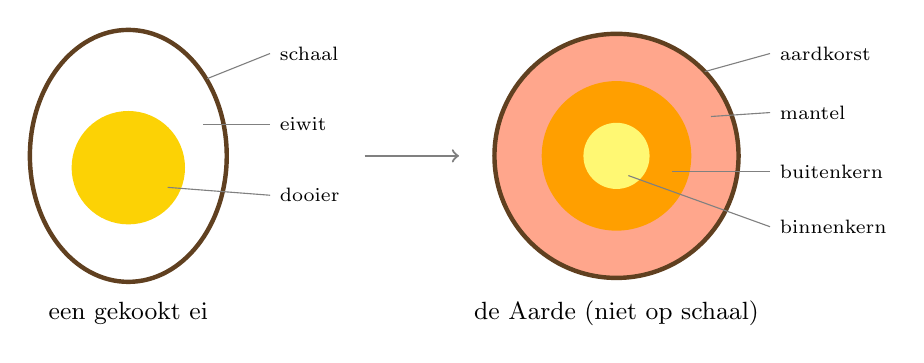
\begin{tikzpicture}
  % a boiled egg cut in half
  \begin{scope}
    \fill[white] (0,0) ellipse (1.25 and 1.6);
    \draw[brown!50!black, line width=1.6pt] (0,0) ellipse (1.25 and 1.6);
    \fill[yellow!70!orange] (0,-0.15) circle (0.72);
    \node[font=\scriptsize, anchor=west] (s) at (1.8,1.3) {schaal};
    \draw[gray] (s.west) -- (1.0,0.98);
    \node[font=\scriptsize, anchor=west] (w) at (1.8,0.4) {eiwit};
    \draw[gray] (w.west) -- (0.95,0.4);
    \node[font=\scriptsize, anchor=west] (y) at (1.8,-0.5) {dooier};
    \draw[gray] (y.west) -- (0.5,-0.4);
    \node[font=\small] at (0,-2.0) {een gekookt ei};
  \end{scope}
  \draw[->, thick, gray] (3.0,0) -- (4.2,0);
  % the Earth, not to scale
  \begin{scope}[xshift=6.2cm]
    \fill[orange!45!red!45] (0,0) circle (1.55);
    \fill[orange!75!yellow] (0,0) circle (0.95);
    \fill[yellow!55] (0,0) circle (0.42);
    \draw[brown!50!black, line width=1.6pt] (0,0) circle (1.55);
    \node[font=\scriptsize, anchor=west] (c) at (1.95,1.3) {aardkorst};
    \draw[gray] (c.west) -- (1.12,1.07);
    \node[font=\scriptsize, anchor=west] (m) at (1.95,0.55) {mantel};
    \draw[gray] (m.west) -- (1.2,0.5);
    \node[font=\scriptsize, anchor=west] (o) at (1.95,-0.2) {buitenkern};
    \draw[gray] (o.west) -- (0.7,-0.2);
    \node[font=\scriptsize, anchor=west] (i) at (1.95,-0.9) {binnenkern};
    \draw[gray] (i.west) -- (0.15,-0.25);
    \node[font=\small] at (0,-2.0) {de Aarde (niet op schaal)};
  \end{scope}
\end{tikzpicture}

{\small De Aarde vergeleken met een gekookt ei. Anders dan de dooier heeft
de \omterm{def:g6:inside-the-earth:layers}{kern} twee delen. In deze tekening is de \omterm{def:g6:inside-the-earth:layers}{aardkorst} veel te dik getekend;
de tekening op schaal volgt hierna.}
% ledger: usgs:layers-egg
\end{omfigure}

\begin{definition}[De lagen van de Aarde]\label{def:g6:inside-the-earth:layers}
De Aarde bestaat uit drie hoofdlagen, van het oppervlak naar het
middelpunt:
\begin{itemize}
  \item de \emph{aardkorst}\index{aardkorst}, een dunne buitenlaag van \omterm{def:g3:stones-pebbles-sand:rock}{vast
        gesteente}, enkele kilometers tot enkele tientallen kilometers dik;
  \item de \emph{mantel}\index{mantel}, een dikke laag heet, dicht, \omterm{def:g3:stones-pebbles-sand:rock}{vast
        gesteente}, tot een diepte van ongeveer 2900~km;
  \item de \emph{kern}\index{kern}, gemaakt van metaal, vooral ijzer met wat
        nikkel, van ongeveer 2900~km diep tot het middelpunt. De kern heeft
        twee delen: de \emph{buitenkern}\index{buitenkern}, die vloeibaar
        is, en de \emph{binnenkern}\index{binnenkern}, een vaste bol in het
        midden, met een straal van ongeveer 1220~km.
\end{itemize}
% ledger: usgs:layers-egg, usgs:crust-thickness, data:prem, earth:Rmean
\end{definition}

De tekening hieronder laat de lagen \emph{op schaal} zien, met de grenzen
zoals die met aardbevingsgolven zijn gemeten.

\begin{omfigure}
\pgfplotstableread{figdata/out/grade-6-earth_layers-disc.dat}\disctab
\pgfplotstablegetelem{0}{r_cm}\of\disctab \let\rE\pgfplotsretval
\pgfplotstablegetelem{1}{r_cm}\of\disctab \let\rOC\pgfplotsretval
\pgfplotstablegetelem{2}{r_cm}\of\disctab \let\rIC\pgfplotsretval
\begin{minipage}[c]{0.43\linewidth}\centering
\begin{tikzpicture}
  \fill[orange!45!red!45] (0,0) circle (\rE cm);
  \fill[orange!75!yellow] (0,0) circle (\rOC cm);
  \fill[yellow!55] (0,0) circle (\rIC cm);
  \draw[brown!50!black, line width=0.45pt] (0,0) circle (\rE cm);
  
  \draw[gray, thin] (-0.25,\rE) rectangle (0.25,\rE-0.12);
  
  \node[font=\scriptsize, align=center, inner sep=0pt] at (0,0) {binnen-\\ kern};
  \node[font=\scriptsize, align=center] at (0,1.03) {buiten-\\ kern};
  \node[font=\scriptsize] at (0,2.12) {mantel};
  \draw[<-, font=\scriptsize] (1.98,1.98) -- (2.3,2.75) node[above, align=center] {aardkorst\\ (een haarlijn)};
\end{tikzpicture}
\end{minipage}\hfill
\begin{minipage}[c]{0.55\linewidth}\centering
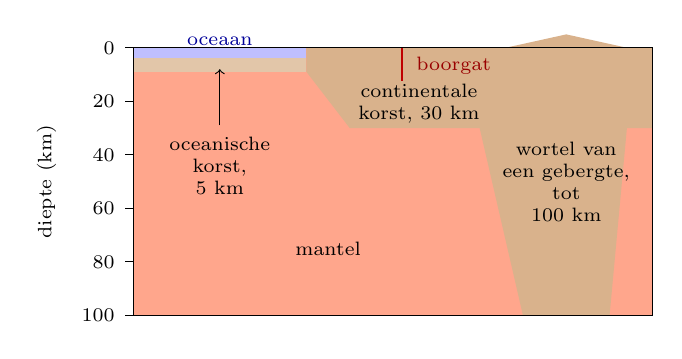
\begin{tikzpicture}[yscale=0.034, xscale=0.55]
  % the top 100 km enlarged: ocean on the left, continent and a range on the right
  \fill[orange!45!red!45] (0,0) rectangle (12,-100);
  \fill[blue!25] (0,0) rectangle (4,-4);
  \fill[brown!45] (0,-4) rectangle (4,-9);                 % oceanic crust 5 km
  \fill[brown!60] (4,0) -- (4,-9) -- (5,-30) -- (8,-30) -- (9,-100) -- (11,-100) -- (11.4,-30) -- (12,-30) -- (12,0) -- cycle;
  \fill[brown!60] (8.6,0) -- (10,5) -- (11.4,0) -- cycle;   % the range (not to scale above ground)
  \draw[red!75!black, line width=0.8pt] (6.2,0) -- (6.2,-12.262);
  \draw[thin] (0,0) rectangle (12,-100);
  \foreach \y in {0,-20,-40,-60,-80,-100} \draw (0,\y) -- (-0.2,\y) node[left, font=\scriptsize] {\pgfmathparse{-\y}\pgfmathprintnumber{\pgfmathresult}};
  \node[font=\scriptsize, rotate=90] at (-2.0,-50) {diepte (km)};
  \node[font=\scriptsize, align=center] at (2,-44) {oceanische\\ korst,\\ 5~km};
  \draw[->, thin] (2,-29) -- (2,-8);
  \node[font=\scriptsize, align=center] at (6.6,-21) {continentale\\ korst, 30~km};
  \node[font=\scriptsize, align=center] at (10.0,-50) {wortel van\\ een gebergte,\\ tot\\ 100~km};
  \node[font=\scriptsize, align=center, red!60!black] at (7.4,-6.5) {boorgat};
  \node[font=\scriptsize] at (4.5,-75) {mantel};
  \node[font=\scriptsize, blue!60!black] at (2,2.5) {oceaan};
\end{tikzpicture}
\end{minipage}

\smallskip
{\small Links: de opengesneden Aarde, op schaal; het kleine grijze vak
bovenaan geeft het deel aan dat rechts is vergroot. Rechts: de bovenste
100~km, ongeveer 60~keer vergroot: dunne korst onder de \omterm{def:g2:water-on-earth:ocean}{oceanen}, dikkere
korst onder de \omterm{def:g3:continents-and-oceans:continent}{continenten}, het dikst onder hoge \omterm{def:g4:world-physical-map:range}{gebergten}; het
recordboorgat in rood.}
% ledger: data:prem, earth:Rmean, usgs:crust-thickness, sciam:kola-depth (figdata/grade-6/earth_layers.py)
\end{omfigure}

\begin{center}\small
\begin{tabular}{|l|c|c|c|l|}
\hline
\textbf{laag} & \textbf{van (km)} & \textbf{tot (km)} & \textbf{dikte (km)} & \textbf{gemaakt van} \\
\hline
\omterm{def:g6:inside-the-earth:layers}{aardkorst} & 0 & 5 tot 100 & 5 tot 100 & \omterm{def:g3:stones-pebbles-sand:rock}{vast gesteente} \\
\omterm{def:g6:inside-the-earth:layers}{mantel} & onderkant van de korst & 2891 & ongeveer 2860 & \omterm{def:g3:stones-pebbles-sand:rock}{vast gesteente}, heel heet \\
\omterm{def:g6:inside-the-earth:layers}{buitenkern} & 2891 & 5150 & ongeveer 2260 & vloeibaar metaal \\
\omterm{def:g6:inside-the-earth:layers}{binnenkern} & 5150 & 6371 (middelpunt) & ongeveer 1220 & vast metaal \\
\hline
\end{tabular}
\end{center}
% ledger: data:prem, usgs:crust-thickness, usgs:layers-egg, earth:Rmean (figdata/grade-6/earth_layers.py, main table)

\textbf{De \omterm{def:g6:inside-the-earth:layers}{aardkorst}} is de enige laag waarop we kunnen lopen en waarin we
kunnen graven. Ze is heel dun vergeleken met de andere: onder de \omterm{def:g2:water-on-earth:ocean}{oceanen}
is ze maar ongeveer 5~km dik; onder de \omterm{def:g3:continents-and-oceans:continent}{continenten} gemiddeld ongeveer
30~km; onder hoge \omterm{def:g4:world-physical-map:range}{gebergten} zoals de Alpen kan haar onderkant wel 100~km
diep liggen, zoals de wortel van een tand. Zelfs het recordboorgat, 12.3~km diep, kwam nog niet halverwege door een gemiddelde continentale korst. Op de tekening op schaal
is de \omterm{def:g6:inside-the-earth:layers}{aardkorst} dunner dan de lijn rond de schijf.
% ledger: usgs:crust-thickness, sciam:kola-depth

\textbf{De \omterm{def:g6:inside-the-earth:layers}{mantel}} is de dikste laag: hij loopt van de onderkant van de
korst tot 2891~km diep, ongeveer 45~\% van de weg naar het middelpunt. Zijn
\omterm{def:g3:stones-pebbles-sand:rock}{gesteente} is vast, maar heel heet en dichter dan het \omterm{def:g3:stones-pebbles-sand:rock}{gesteente} van de
korst. In miljoenen jaren kan het hete \omterm{def:g3:stones-pebbles-sand:rock}{gesteente} van een deel van de \omterm{def:g6:inside-the-earth:layers}{mantel}
heel langzaam kruipen, als een heel stijve pasta.
% ledger: data:prem, usgs:layers-egg, usgs:lithosphere-80km

\textbf{De \omterm{def:g6:inside-the-earth:layers}{kern}} begint op 2891~km en loopt door tot het middelpunt. Hij
bestaat niet uit \omterm{def:g3:stones-pebbles-sand:rock}{gesteente} maar uit metaal: een legering van ijzer en
nikkel, bijna twee keer zo dicht als de \omterm{def:g6:inside-the-earth:layers}{mantel}. Zijn buitenste deel is
\emph{vloeibaar}: een \omterm{def:g2:water-on-earth:ocean}{oceaan} van gesmolten metaal van meer dan 2000~km
diep. Zijn binnenste deel, van 5150~km tot het middelpunt, is een
\emph{vaste} bol van metaal met een straal van ongeveer 1220~km: ongeveer 70~\% zo breed als de Maan. Terwijl de Aarde draait, beweegt het vloeibare metaal van de
\omterm{def:g6:inside-the-earth:layers}{buitenkern}, en die beweging maakt het magnetisch veld van de Aarde, het
veld dat een kompasnaald laat draaien.
% ledger: data:prem, usgs:layers-egg, earth:Rmean, planet:Moon.diameter

Hoe dieper, hoe dichter. Water heeft een dichtheid van 1~gram per kubieke
centimeter: het \omterm{def:g3:stones-pebbles-sand:rock}{gesteente} van de \omterm{def:g6:inside-the-earth:layers}{aardkorst} is 2.6 tot 2.9 keer zo dicht,
het \omterm{def:g3:stones-pebbles-sand:rock}{gesteente} onder in de \omterm{def:g6:inside-the-earth:layers}{mantel} meer dan 5~keer, en het metaal in het
middelpunt ongeveer 13~keer (zie de grafiek hieronder). De zwaarste materialen zitten in het midden en de lichtste bovenop: de Aarde is gesorteerd, van de lichte korst tot de zware metalen \omterm{def:g6:inside-the-earth:layers}{kern}.
% ledger: data:prem


\begin{omfigure}
\begin{tikzpicture}
  \begin{axis}[omrecord, width=0.86\linewidth, height=5.4cm,
      xmin=0, xmax=6371, ymin=0, ymax=14,
      xlabel={diepte onder het oppervlak (km)},
      ylabel={dichtheid (g per cm$^3$)},
      xtick={0,1000,2000,3000,4000,5000,6000},
      scaled x ticks=false, x tick label style={/pgf/number format/1000 sep={}},
      clip=false]
    \fill[orange!45!red!20] (axis cs:24.4,0) rectangle (axis cs:2891,14);
    \fill[orange!75!yellow!35] (axis cs:2891,0) rectangle (axis cs:5149.5,14);
    \fill[yellow!30] (axis cs:5149.5,0) rectangle (axis cs:6371,14);
    \addplot[very thick, black] table[x=depth_km, y=rho] {figdata/out/grade-6-earth_layers-profile.dat};
    \node[font=\scriptsize] at (axis cs:1450,12.5) {mantel};
    \node[font=\scriptsize] at (axis cs:4020,4.5) {buitenkern};
    \node[font=\scriptsize] at (axis cs:5760,4.5) {binnenkern};
    \node[font=\scriptsize, align=left, anchor=west] at (axis cs:80,1.4) {aardkorst: 2.6 tot 2.9};
  \end{axis}
\end{tikzpicture}

{\small Hoe dicht de Aarde op elke diepte is, volgens een referentiemodel
dat uit aardbevingsmetingen is opgebouwd. De dichtheid springt van ongeveer
5.6 naar ongeveer 9.9~g per cm$^3$ waar het \omterm{def:g3:stones-pebbles-sand:rock}{gesteente} van de \omterm{def:g6:inside-the-earth:layers}{mantel}
overgaat in het metaal van de \omterm{def:g6:inside-the-earth:layers}{kern}.}
% ledger: data:prem (figdata/grade-6/earth_layers.py, part profile)
\end{omfigure}

\begin{inthelab}[Lagen in een glas (in de klas, met de leraar)]
De leraar giet langzaam en na elkaar in een hoog glas: wat honing, wat
water gekleurd met een druppel inkt, en wat slaolie. In welke volgorde er
ook wordt gegoten, na een tijdje ligt de honing onderop, het water in het
midden en de olie bovenop: elke vloeistof zakt onder de lichtere en blijft
boven de dichtere. Geschud wordt het glas troebel; laat je het staan, dan
sorteert het zichzelf weer. De Aarde is op dezelfde manier gelaagd: het dichtste materiaal, het metaal van de \omterm{def:g6:inside-the-earth:layers}{kern}, zit in het midden, en het lichtste \omterm{def:g3:stones-pebbles-sand:rock}{gesteente} bovenop.
\end{inthelab}


\begin{remark}[Hoe dun is de aardkorst?]\label{rem:g6:inside-the-earth:thin-crust}
Op een schoolglobe van 30~cm doorsnede zou de continentale korst (30~km)
ongeveer 0.7~millimeter dik zijn, en de oceanische korst (5~km) ongeveer zo
dik als een vel papier. De \omterm{def:g6:inside-the-earth:layers}{aardkorst} is minder dan een half procent van
de straal: $30 \div 6371 \approx 0.0047$, dat is 0.47~\%.
% ledger: usgs:crust-thickness, earth:Rmean
\end{remark}

\section{Hoe aardbevingsgolven ons de rest vertellen}\label{sec:g6:inside-the-earth:waves}

Als niemand dieper is geweest dan 12~km, hoe kunnen we de \omterm{def:g6:inside-the-earth:layers}{kern} dan tekenen?
Het antwoord komt van \omterm{def:g4:volcanoes-earthquakes-first-look:earthquake}{aardbevingen}. Als een \omterm{def:g4:volcanoes-earthquakes-first-look:earthquake}{aardbeving} de grond doet
schudden, vertrekken er golven in alle richtingen, die \emph{door} de hele
Aarde reizen, zoals het geluid van een klop door een muur reist. Instrumenten op veel plaatsen in de wereld registreren wanneer elke golf aankomt (je leert ze kennen in
\cref{ch:g7:earthquakes}).
% ledger: data:prem

De golven reizen niet in elk materiaal even snel. Als ze de grens tussen
twee lagen bereiken, verandert hun snelheid plotseling: sommige golven
kaatsen terug, andere buigen af als ze de grens oversteken, een beetje
zoals licht dat water binnengaat. Door de golven van veel \omterm{def:g4:volcanoes-earthquakes-first-look:earthquake}{aardbevingen} te timen, bij meetstations over de hele wereld, hebben wetenschappers gevonden waar die grenzen liggen,
en welke lagen vast of vloeibaar zijn. Seismologen noemen de twee
belangrijkste soorten golven \emph{P-golven} (de snellere, die het
\omterm{def:g3:stones-pebbles-sand:rock}{gesteente} samendrukken en uitrekken) en \emph{S-golven} (de langzamere,
die het heen en weer schudden); latere delen bestuderen ze nauwkeurig. De
S-golven hebben één opvallende eigenschap: ze kunnen niet door een
vloeistof reizen.

\begin{omfigure}
\begin{tikzpicture}
  \begin{axis}[omrecord, width=0.86\linewidth, height=5.4cm,
      xmin=0, xmax=6371, ymin=0, ymax=14.5,
      xlabel={diepte onder het oppervlak (km)},
      ylabel={golfsnelheid (km per seconde)},
      xtick={0,1000,2000,3000,4000,5000,6000},
      scaled x ticks=false, x tick label style={/pgf/number format/1000 sep={}},
      clip=false]
    \fill[orange!45!red!20] (axis cs:24.4,0) rectangle (axis cs:2891,14.5);
    \fill[orange!75!yellow!35] (axis cs:2891,0) rectangle (axis cs:5149.5,14.5);
    \fill[yellow!30] (axis cs:5149.5,0) rectangle (axis cs:6371,14.5);
    \addplot[very thick, blue!70!black] table[x=depth_km, y=vp] {figdata/out/grade-6-earth_layers-profile.dat};
    \addplot[very thick, red!75!black] table[x=depth_km, y=vs] {figdata/out/grade-6-earth_layers-profile.dat};
    \node[font=\scriptsize, blue!70!black, anchor=south] at (axis cs:1300,12.9) {P-golven (sneller)};
    \node[font=\scriptsize, red!75!black, anchor=north] at (axis cs:1500,6.1) {S-golven (langzamer)};
    \node[font=\scriptsize, red!75!black, align=center, fill=white, fill opacity=0.8, text opacity=1] at (axis cs:4020,1.9) {S-golven: 0\\ (vloeibaar)};
    \node[font=\scriptsize] at (axis cs:4020,13.6) {buitenkern};
    \node[font=\scriptsize] at (axis cs:5760,13.6) {binnenkern};
    \node[font=\scriptsize] at (axis cs:1450,1.5) {mantel};
  \end{axis}
\end{tikzpicture}

{\small De snelheid van de twee soorten aardbevingsgolven op elke diepte, in
hetzelfde referentiemodel. In de \omterm{def:g6:inside-the-earth:layers}{buitenkern} stoppen de S-golven: hun
snelheid is nul, omdat de \omterm{def:g6:inside-the-earth:layers}{buitenkern} vloeibaar is.}
% ledger: data:prem (figdata/grade-6/earth_layers.py, part profile)
\end{omfigure}

De grafiek van links naar rechts gelezen: in de \omterm{def:g6:inside-the-earth:layers}{mantel} gaan beide soorten
golven steeds sneller naarmate het dieper wordt. Op 2891~km verdwijnen de
S-golven en worden de P-golven plotseling langzamer: dat is de bovenkant
van de vloeibare \omterm{def:g6:inside-the-earth:layers}{buitenkern}. Op 5150~km worden de P-golven weer sneller en
bestaan er weer S-golven: dat is de vaste \omterm{def:g6:inside-the-earth:layers}{binnenkern}.
% ledger: data:prem

\begin{history}[Inge Lehmann en de binnenkern]
\begin{minipage}[c]{0.72\linewidth}
Begin jaren dertig dachten seismologen dat de Aarde twee lagen had: een vaste \omterm{def:g6:inside-the-earth:layers}{mantel} rond een vloeibare \omterm{def:g6:inside-the-earth:layers}{kern}. De Deense seismologe Inge Lehmann bestudeerde de golven van een
zware \omterm{def:g4:volcanoes-earthquakes-first-look:earthquake}{aardbeving} die Nieuw-Zeeland in 1929 trof, geregistreerd bij
meetstations ver weg. Sommige golven kwamen aan op plaatsen waar ze bij
een volledig vloeibare \omterm{def:g6:inside-the-earth:layers}{kern} helemaal niet hadden mogen aankomen. In een
artikel uit 1936, eenvoudig ``P\,$'$'' genoemd, stelde ze een verklaring
voor: in de vloeibare \omterm{def:g6:inside-the-earth:layers}{kern} zit een kleinere \emph{vaste \omterm{def:g6:inside-the-earth:layers}{binnenkern}}, die
deze golven terugkaatst. Ze schreef bescheiden dat de gegevens ``ruim
onvoldoende'' waren om zeker te zijn, maar dat de verklaring ``mogelijk
lijkt'', en ze vroeg andere onderzoekers om haar te toetsen. Dat deden ze, en nu hoort de vaste \omterm{def:g6:inside-the-earth:layers}{binnenkern} bij elk referentiemodel van de Aarde, zoals het model dat in de grafieken van dit hoofdstuk is gebruikt.
% ledger: nbi:lehmann-1936
\end{minipage}\hfill
\begin{minipage}[c]{0.24\linewidth}\centering
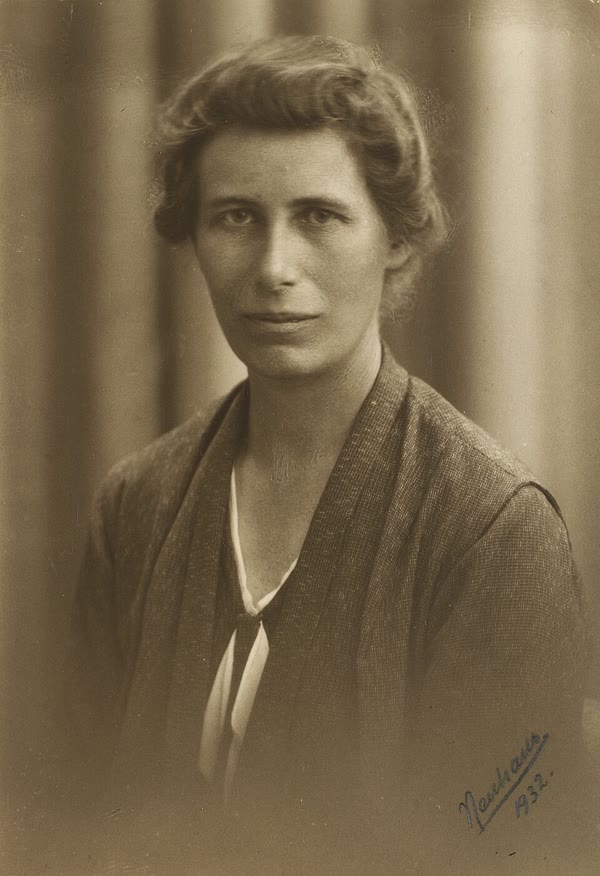
\includegraphics[width=\linewidth]{images/book1/g6-inge-lehmann.jpg}\\[2pt]
{\footnotesize Inge Lehmann in 1932. (Foto: Even Neuhaus, publiek domein,
via Wikimedia Commons.)}
% ledger: commons:inge-lehmann
\end{minipage}
\end{history}

\section{Hoe dieper, hoe heter}

Elke diepe mijn en elk diep boorgat laat hetzelfde zien: hoe dieper je
gaat, hoe heter het \omterm{def:g3:stones-pebbles-sand:rock}{gesteente}. In de diepste mijn worden de rotswanden
ongeveer 60~graden Celsius, meer dan 4~km diep; onder in het
recordboorgat, 12.3~km diep, was het \omterm{def:g3:stones-pebbles-sand:rock}{gesteente} ongeveer 180~graden.
% ledger: gwr:deepest-mine, sciam:kola-180C

Dicht bij het oppervlak stijgt de temperatuur in een vrij vast tempo. In
de Verenigde Staten verzamelden wetenschappers de metingen van
284~boorgaten, de meeste dieper dan 600~m. Gemiddeld steeg de temperatuur
met \textbf{29~graden per kilometer} diepte: ongeveer 25~graden per
kilometer in het oosten van het land en 34 in het westen. Maar het tempo
verschilt sterk van plaats tot plaats: in die boorgaten liep het van 6 tot
69~graden per kilometer.
% ledger: usgs:gradient-29

\begin{omfigure}
\begin{tikzpicture}
  \begin{axis}[omrecord, omdepth, width=0.78\linewidth, height=5.6cm,
      xmin=0, xmax=160, ymin=0, ymax=2,
      xlabel={temperatuur van het gesteente ($^\circ$C)},
      ylabel={diepte (km)},
      ytick={0,0.5,1,1.5,2},
      yticklabel style={/pgf/number format/fixed},
      legend pos=north east, legend cell align=left,
            legend style={font=\scriptsize},
      clip=false]
    \addplot[forget plot, name path=lo, thin, gray] table[x=t_low, y=depth_km] {figdata/out/grade-6-earth_layers-geotherm.dat};
    \addplot[forget plot, name path=hi, thin, gray] table[x=t_high, y=depth_km] {figdata/out/grade-6-earth_layers-geotherm.dat};
    \addplot[forget plot, gray!20] fill between[of=lo and hi];
    \addplot[forget plot, thick, blue!70!black] table[x=t_east, y=depth_km] {figdata/out/grade-6-earth_layers-geotherm.dat};
    \addplot[forget plot, very thick, black] table[x=t_mean, y=depth_km] {figdata/out/grade-6-earth_layers-geotherm.dat};
    \addplot[forget plot, thick, red!75!black] table[x=t_west, y=depth_km] {figdata/out/grade-6-earth_layers-geotherm.dat};
    \addlegendimage{area legend, fill=gray!20, draw=gray}
    \addlegendentry{6 tot 69 $^\circ$C per km: alle boorgaten}
    \addlegendimage{thick, blue!70!black}\addlegendentry{25 $^\circ$C per km: oosten}
    \addlegendimage{very thick, black}\addlegendentry{29 $^\circ$C per km: gemiddeld}
    \addlegendimage{thick, red!75!black}\addlegendentry{34 $^\circ$C per km: westen}
  \end{axis}
\end{tikzpicture}

{\small De temperatuur tegen de diepte (naar beneden) voor een bodem die op
15~$^\circ$C begint, bij het gemiddelde tempo (29, zwart), de gemiddelden
van het oosten en het westen (25 en 34) en het hele gemeten bereik (6 tot
69, grijze band). De metingen gaan tot ongeveer 2~km.}
% ledger: usgs:gradient-29, planet:Earth.Tmean (figdata/grade-6/earth_layers.py, part geotherm)
\end{omfigure}

\begin{method}[Temperatuur op een bepaalde diepte]\label{met:g6:inside-the-earth:temperature}
\begin{enumerate}
  \item Neem de temperatuur van de bodem dicht bij het oppervlak.
  \item Vermenigvuldig de diepte, in kilometer, met het tempo, in graden
        per kilometer: zoveel warmer wordt het.
  \item Tel de twee op. Gebruik dit alleen binnen het bereik waarin het
        tempo is gemeten: een paar kilometer.
\end{enumerate}
\end{method}

\begin{example}[Twee kilometer diep]\label{ex:g6:inside-the-earth:two-km}
De bodem is 15~$^\circ$C en het tempo is 29~graden per kilometer. Op 2~km:
$2 \times 29 = 58$ graden warmer, dus $15 + 58 = 73~^\circ$C: heter dan het
heetste bad, en al veel te heet om aan te raken.
% ledger: usgs:gradient-29, planet:Earth.Tmean
\end{example}

Kan hetzelfde tempo helemaal tot het middelpunt worden gebruikt? Nee. Bij
29~graden per kilometer zou het middelpunt ongeveer 185\,000~graden zijn,
en dat is onmogelijk: het tempo dat in de eerste kilometers is gemeten, geldt niet diep onder de grond, waar de stijging veel langzamer moet zijn. Wetenschappers schatten de
temperatuur van de \omterm{def:g6:inside-the-earth:layers}{kern} op een andere manier: in het laboratorium knijpen
ze piepkleine korreltjes ijzer tussen twee diamanten samen, tot miljoenen
keren de luchtdruk, en verhitten ze met lasers tot ze smelten. Zo vonden
ze dat de temperatuur aan de rand van de vaste \omterm{def:g6:inside-the-earth:layers}{binnenkern} ongeveer
\textbf{6000~graden Celsius} is, en toch blijft het ijzer van de \omterm{def:g6:inside-the-earth:layers}{binnenkern} vast, omdat de druk daar, ongeveer
3.3~miljoen keer de luchtdruk, het belet te smelten.
% ledger: esrf:core-6000C, usgs:gradient-29

\begin{remark}[Heet, en toch vast]\label{rem:g6:inside-the-earth:pressure}
Als je een stof hard samenperst, smelt ze pas bij een hogere temperatuur.
De \omterm{def:g6:inside-the-earth:layers}{mantel} is heel heet, maar blijft vast; de \omterm{def:g6:inside-the-earth:layers}{buitenkern} is vloeibaar; de
\omterm{def:g6:inside-the-earth:layers}{binnenkern}, nog heter, is weer vast, omdat die het hardst van allemaal
wordt samengeperst. Of iets smelt of niet, hangt af van de temperatuur
\emph{en} van de druk.
% ledger: esrf:core-6000C, data:prem
\end{remark}

\section{Oefeningen}

\begin{exercise}[$\star$]\label{exo:g6:inside-the-earth:1}
Noem de vier lagen van de Aarde op volgorde, van het oppervlak naar het
middelpunt. Welke is vloeibaar? Welke zijn van metaal?
\end{exercise}

\begin{exercise}[$\star$]\label{exo:g6:inside-the-earth:2}
Waar of niet waar? Verbeter de zinnen die niet waar zijn.
(a) De \omterm{def:g6:inside-the-earth:layers}{aardkorst} is dikker onder de \omterm{def:g2:water-on-earth:ocean}{oceanen} dan onder de \omterm{def:g3:continents-and-oceans:continent}{continenten}.
(b) De \omterm{def:g6:inside-the-earth:layers}{kern} is van \omterm{def:g3:stones-pebbles-sand:rock}{gesteente}.
(c) De \omterm{def:g6:inside-the-earth:layers}{binnenkern} is vast.
(d) Het diepste boorgat dat ooit is gegraven, is ongeveer 12~km diep.
\end{exercise}

\begin{exercise}[$\star$]\label{exo:g6:inside-the-earth:3}
Gebruik de tabel van de lagen. (a) Op welke diepte begint de \omterm{def:g6:inside-the-earth:layers}{kern}?
(b) Op welke diepte begint de \omterm{def:g6:inside-the-earth:layers}{binnenkern}? (c) Hoe dik is de \omterm{def:g6:inside-the-earth:layers}{buitenkern}?
\end{exercise}

\begin{exercise}[$\star$]\label{exo:g6:inside-the-earth:4}
De Aarde wordt vaak vergeleken met een gekookt ei. Neem over en vul aan:
``De schaal is als de \ldots, het eiwit is als de \ldots{} en de dooier is
als de \ldots{}. Maar anders dan de dooier heeft de \ldots{} twee delen: een
vloeibare \ldots{} en een vaste \ldots{}.''
\end{exercise}

\begin{exercise}[$\star\star$]\label{exo:g6:inside-the-earth:5}
Mount Everest is 8.849~km hoog en de straal van de Aarde is 6371~km.
Hoe hoog is Everest als percentage van de straal? Rond af op twee
decimalen. Is het aardoppervlak, van ver gezien, erg hobbelig?
\end{exercise}

\begin{exercise}[$\star\star$]\label{exo:g6:inside-the-earth:6}
De continentale korst is gemiddeld 30~km dik en de oceanische korst 5~km.
(a) Hoeveel keer dikker is de continentale korst? (b) Onder een hoog
\omterm{def:g4:world-physical-map:range}{gebergte} kan de korst 100~km dik worden. Hoeveel keer dikker dan de
oceanische korst is dat?
\end{exercise}

\begin{exercise}[$\star\star$]\label{exo:g6:inside-the-earth:7}
In een gebied is de bodem 12~$^\circ$C en stijgt de temperatuur met
25~graden per kilometer. Wat is de temperatuur (a) op 1~km, (b) op
1.5~km, (c) op 2~km?
\end{exercise}

\begin{exercise}[$\star\star$]\label{exo:g6:inside-the-earth:8}
In een boorgat is het \omterm{def:g3:stones-pebbles-sand:rock}{gesteente} 14~$^\circ$C dicht bij het oppervlak en
74~$^\circ$C op een diepte van 2~km. Met hoeveel graden stijgt de
temperatuur per kilometer? Ligt dit tempo tussen de gemiddelden van het
oosten en het westen uit de metingen van het hoofdstuk?
\end{exercise}

\begin{exercise}[$\star\star$]\label{exo:g6:inside-the-earth:9}
Gebruik de grafiek van de golfsnelheden. (a) Wat is de snelheid van de
P-golven vlak boven de \omterm{def:g6:inside-the-earth:layers}{kern}, op ongeveer 2890~km, en vlak onder de
bovenkant van de \omterm{def:g6:inside-the-earth:layers}{kern}? (b) Tussen welke diepten is de snelheid van de
S-golven nul? (c) Wat zegt dat over die laag?
\end{exercise}

\begin{exercise}[$\star\star$]\label{exo:g6:inside-the-earth:10}
Het recordboorgat is 12.3~km diep. (a) Welk percentage van een gemiddelde
continentale korst (30~km) is erdoorheen geboord? (b) Bereikte het de
\omterm{def:g6:inside-the-earth:layers}{mantel}?
\end{exercise}

\begin{exercise}[$\star\star\star$]\label{exo:g6:inside-the-earth:11}
Leo zegt: ``Dicht bij het oppervlak stijgt de temperatuur met 29~graden
per kilometer, dus in het middelpunt, 6371~km diep, moet het
$15 + 29 \times 6371$ graden zijn.'' (a) Bereken het getal van Leo.
(b) Vergelijk het met de temperatuur die in het laboratorium is gevonden
voor de rand van de \omterm{def:g6:inside-the-earth:layers}{binnenkern}. (c) Wat is er mis met de redenering van
Leo?
\end{exercise}

\begin{exercise}[$\star\star\star$]\label{exo:g6:inside-the-earth:12}
De hele Aarde heeft een gemiddelde dichtheid van ongeveer 5.5~gram per
kubieke centimeter (\cref{ch:g6:earth-a-planet}), maar de \omterm{def:g3:stones-pebbles-sand:rock}{gesteenten} van de
\omterm{def:g6:inside-the-earth:layers}{aardkorst} hebben een dichtheid van maar 2.6 tot 2.9. (a) Wat zegt dit over
het materiaal dieper in de Aarde? (b) Gebruik de grafiek van de dichtheid:
in welke lagen is de dichtheid overal groter dan 5.5? (c) Waarom is het
logisch dat het zware metaal in het midden ligt en niet aan het oppervlak?
\end{exercise}

\section{Probleem: Een reis naar het middelpunt, op schaal}

\begin{problem}[{Weekendprobleem --- een model van de Aarde van 2~meter
doorsnede: de lagen, de diepste gaten en het hete binnenste, op schaal}]
\label{pb:g6:inside-the-earth:1}
% ledger: earth:Rmean, data:prem, usgs:crust-thickness, sciam:kola-depth, tht:everest, usgs:gradient-29, gwr:deepest-mine, esrf:core-6000C
Voor de schoolmarkt bouwt een klas een model van de Aarde, doormidden
gesneden, zo groot mogelijk: het platte vlak van de halve bol is een schijf
van 2~meter doorsnede, beschilderd met de lagen. Alles moet op schaal zijn.
Gebruik: straal van de Aarde 6371~km; bovenkant van de \omterm{def:g6:inside-the-earth:layers}{buitenkern}
2891~km; bovenkant van de \omterm{def:g6:inside-the-earth:layers}{binnenkern} 5150~km; continentale korst 30~km;
oceanische korst 5~km; Everest 8.849~km; recordboorgat 12.3~km.

\medskip
\noindent\textbf{Deel I --- Het model.}
\begin{enumerate}
  \item Wat is de diameter van de Aarde, in kilometer? Schrijf de diameter
        van het model in millimeter.
  \item Voor hoeveel kilometer van de echte Aarde staat 1~millimeter van
        het model? (Deel de echte diameter door de diameter van het model.)
  \item Hoe hoog is Everest op het model, in millimeter? Rond af op één
        decimaal.
  \item Hoe diep is het recordboorgat op het model? Vergelijk het met de
        afstand van het oppervlak tot het middelpunt van het model.
\end{enumerate}

\medskip
\noindent\textbf{Deel II --- De lagen.}
\begin{enumerate}[resume]
  \item Op welke afstand onder het oppervlak van het model moeten de
        leerlingen de bovenkant van de \omterm{def:g6:inside-the-earth:layers}{buitenkern} schilderen? Rond af op
        een hele millimeter.
  \item Dezelfde vraag voor de bovenkant van de \omterm{def:g6:inside-the-earth:layers}{binnenkern}. Wat is de straal
        van de \omterm{def:g6:inside-the-earth:layers}{binnenkern} op het model?
  \item Welke laag neemt langs een straal van het model de meeste ruimte
        in: de \omterm{def:g6:inside-the-earth:layers}{mantel}, de \omterm{def:g6:inside-the-earth:layers}{buitenkern} of de \omterm{def:g6:inside-the-earth:layers}{binnenkern}? Geef de dikte ervan
        op het model.
  \item Hoe dik moet de continentale korst worden geschilderd? Rond af op
        één decimaal. Is dat makkelijk met een kwast?
\end{enumerate}

\medskip
\noindent\textbf{Deel III --- Het hete binnenste.}
\begin{enumerate}[resume]
  \item De leerlingen schrijven de temperatuur op 2~km op, met een bodem
        van 15~$^\circ$C en 29~graden per kilometer. Wat schrijven ze op?
        Op welke afstand onder het oppervlak van het model ligt 2~km?
  \item De diepste mijn gaat meer dan 4~km diep. Is de mijn op het model
        dieper of minder diep dan het recordboorgat? Ongeveer hoeveel
        millimeter?
  \item Bij de rand van de \omterm{def:g6:inside-the-earth:layers}{binnenkern} staat op het etiket ``ongeveer
        6000~$^\circ$C, vast''. Een bezoeker is verbaasd: waarom is de
        \omterm{def:g6:inside-the-earth:layers}{buitenkern} vloeibaar, maar de \omterm{def:g6:inside-the-earth:layers}{binnenkern}, die nog heter is, vast?
  \item De oceanische korst is de dunste laag. Hoe dik moet die op het
        model zijn, in millimeter? Rond af op twee decimalen, en vergelijk
        het met de dikte van een vel papier (ongeveer 0.1~mm).
\end{enumerate}
\end{problem}
